\documentclass[13pt]{extarticle}

% \usepackage[T1]{fontenc}
\usepackage[utf8]{inputenc}
\usepackage[russian]{babel}

% page margin
\usepackage[top=2cm, bottom=2cm, left=1cm, right=1cm]{geometry}

% AMS packages
\usepackage{amsmath}
\usepackage{amssymb}
\usepackage{amsfonts}
\usepackage{amsthm}

\usepackage{float}
\usepackage{graphicx}
\usepackage{tabularx}
\usepackage[justification=centering]{caption}

\newcommand{\lb}{\left(}
\newcommand{\rb}{\right)}
\newcommand{\dprime}{{\prime\prime}}

\makeatletter
\setlength{\@fptop}{0pt}
\makeatother

\renewcommand{\arraystretch}{1.2}

\begin{document}

\begin{table}
	\begin{minipage}{0.4\textwidth}
		\centering
		\begin{tabular}{|c|c|c|c|}
			\hline
			J & $\nu \lb P_J \rb$ & $\nu \lb R_J \rb$ & m \\
			\hline
			$13$ & $1934.8$ & & $-13$ \\
			$12$ & $1948.0$ & & $-12$ \\
			$11$ & $1961.0$ & & $-11$ \\
			$10$ & $1973.9$ & & $-10$ \\
			$9$  & $1986.5$ & & $-9$ \\
			$8$  & $1999.0$ & & $-8$ \\
			$7$  & $2011.2$ & & $-7$ \\
			$6$  & $2023.3$ & & $-6$ \\
			$5$  & $2035.2$ & & $-5$ \\
			$4$  & $2046.8$ & & $-4$ \\
			$3$  & $2058.3$ & & $-3$ \\
			$2$  & $2069.5$ & & $-2$ \\
			$1$  & $2080.5$ & & $-1$ \\
			$0$  & & $2101.8$ & $1$ \\
			$1$  & & $2112.2$ & $2$ \\
			$2$  & & $2122.2$ & $3$ \\
			$3$  & & $2132.1$ & $4$ \\
			$4$  & & $2141.7$ & $5$ \\
			$5$  & & $2151.1$ & $6$ \\
			$6$  & & $2160.2$ & $7$ \\
			$7$  & & $2169.2$ & $8$ \\
			$8$  & & $2177.8$ & $9$ \\
			$9$  & & $2186.2$ & $10$ \\
			$10$ & & $2194.3$ & $11$ \\
			$11$ & & $2202.2$ & $12$ \\
			$12$ & & $2209.8$ & $13$ \\
			\hline
		\end{tabular}
	\end{minipage}
	\begin{minipage}{0.6\textwidth}
		\centering
		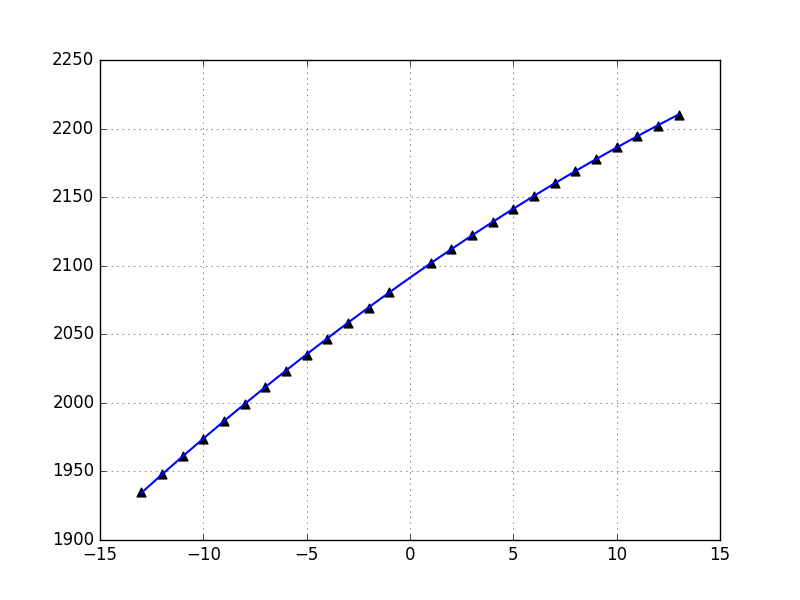
\includegraphics[scale=0.6]{pictures/pic1.png}
				\captionof{figure}{Обработка результатов по ур. (I.2) полосы $0 \rightarrow 1$}
	\end{minipage}
\end{table}

\clearpage
\begin{table}
	\begin{minipage}{0.4\textwidth}
		\begin{tabular}{|c|c|c|c|}
			\hline
			J & $\nu \lb P_J \rb$ & $\nu \lb R_J \rb$ & m \\
			\hline
			$11$ & $3986.2$ & & $-11$ \\
			$10$ & $4001.4$ & & $-10$ \\
			$9$ & $4016.0$ & & $-9$ \\
			$8$ & $4030.3$ & & $-8$ \\
			$7$ & $4044.1$ & & $-7$ \\
			$6$ & $4057.5$ & & $-6$ \\
			$5$ & $4070.5$ & & $-5$ \\
			$4$ & $4083.0$ & & $-4$ \\
			$3$ & $4095.1$ & & $-3$ \\
			$2$ & $4106.8$ & & $-2$ \\
			$1$ & $4118.0$ & & $-1$ \\
			$0$ & & $4139.2$ & $1$ \\
			$1$ & & $4149.0$ & $2$ \\
			$2$ & & $4158.5$ & $3$ \\
			$3$ & & $4167.4$ & $4$ \\
			$4$ & & $4176.0$ & $5$ \\
			$5$ & & $4184.0$ & $6$ \\
			$6$ & & $4191.6$ & $7$ \\
			$7$ & & $4198.8$ & $8$ \\
			$8$ & & $4205.3$ & $9$ \\
			$9$ & & $4211.4$ & $10$ \\
			$10$ & & $4217.1$ & $11$ \\
			\hline
		\end{tabular}
	\end{minipage}
	\begin{minipage}{0.6\textwidth}
		%\centering
		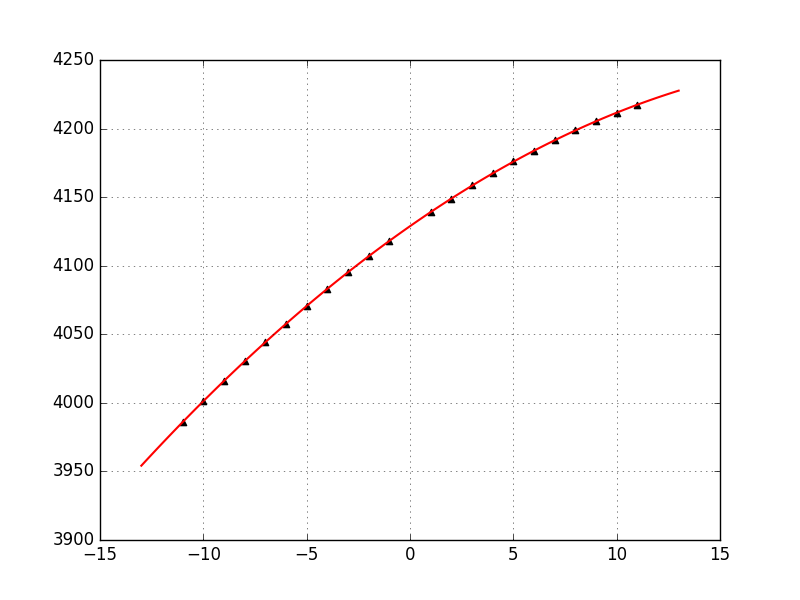
\includegraphics[scale=0.6]{pictures/pic2.png}
		 \captionof{figure}{Обработка результатов по ур. (I.2) полосы $0 \rightarrow 2$}
	\end{minipage}
\end{table}

\clearpage

\section{Отнесение колебательного спектра}
\begin{gather}
	\nu \lb 1 \rightarrow 0 \rb = 2088.15 \textup{см}^{-1}, \nu \lb 2 \rightarrow 0 \rb = 4122.75 \textup{см}^{-1} \notag \\
	\begin{aligned}
		\nu \lb 1 \rightarrow 0 \rb &= \omega_e - 2 \omega_e x_e \\
		\nu \lb 2 \rightarrow 0 \rb &= 2 \omega_e - 6 \omega_e x_e 
	\end{aligned}
	\quad \implies \quad
	\begin{aligned}
		\omega_e &= 3 \nu \lb 1 \rightarrow 0 \rb - \nu \lb 2 \rightarrow 0 \rb = 2141.70 \textup{см}^{-1}\\
		\omega_e x_e &= \frac{1}{2} \lb 2 \nu \lb 1 \rightarrow 0 \rb - \nu \lb 2 \rightarrow 0 \rb \rb = 26.775 \textup{см}^{-1}
	\end{aligned} \notag \\
	v_{max} + \frac{1}{2} = \frac{\omega_e}{2 \omega_e x_e} \quad \implies \quad v_{max} = 39 \notag \\
	D_e = E_{v_{max}} = \omega_e \lb v_{max} + \frac{1}{2} \rb - \omega_e x_e \lb v_{max} + \frac{1}{2} \rb^2 = 42821.46 \textup{см}^{-1} = 5.309 \, \textup{эВ} \notag
\end{gather}

\section{Анализ вращательной структуры колебательных полос}

В приближении жесткого ротатора:
\begin{gather}
\nu_P \lb \nu^\prime, \nu^{\prime\prime}, J \rb = E^\prime \lb \nu^\prime, J - 1 \rb - E^{\prime\prime}\lb \nu^{\dprime}, J \rb \approx \notag \nu_{\nu^\prime,\nu^\dprime} - \lb B^\prime + B^\dprime \rb J + \lb B^\prime - B^\dprime \rb J^2 \notag \\
\nu_R \lb \nu^\prime, \nu^\dprime, J \rb = E^\prime \lb \nu^\prime, J + 1 \rb - E^\dprime \lb \nu^\dprime, J \rb \approx \nu_{\nu^\prime, \nu^\dprime} + \lb B^\prime + B^\dprime \rb \lb J + 1 \rb + \lb B^\prime - B^\dprime \rb \lb J + 1 \rb^2 \notag \\
\nu \lb \nu^\prime, \nu^\dprime, J \rb = \nu_{\nu^\prime, \nu^\dprime} + \lb B^\prime + B^\dprime \rb m + \lb B^\prime - B^\dprime \rb m^2 = \nu_{\nu^\prime, \nu^\dprime} + c_1 m + c_2 m^2 \notag \\
\begin{aligned}
	B^\prime = \frac{1}{2} \lb c_1 + c_2 \rb \\
	B^\dprime = \frac{1}{2} \lb c_1 - c_2 \rb
\end{aligned} \notag
\end{gather} 
С учетом центробежного искажения:
\begin{gather}
E_{\nu, J} = E_{vib} + B_v \lb J \lb J + 1 \rb \rb - D_v \left[ J \lb J + 1 \rb \right]^2 \notag \\
\nu \lb \nu^\prime, \nu^\dprime, J \rb = \nu_{\nu^\prime, \nu^\dprime} + \lb B^\prime + B^\dprime \rb m + \lb B^\prime - B^\dprime - D^\prime + D^\dprime \rb m^2 - 2 \lb D^\prime + D^\dprime \rb m^3 - \lb D^\prime - D^\dprime \rb m^4  = \notag \\
= \nu_{\nu^\prime, \nu^\dprime} + c_1 m + c_2 m^2 + c_3 m^3 + c_4 m^4 \notag \\ 
\begin{aligned}
	D^\prime = -\frac{1}{2} c_4 - \frac{1}{4} c_3 \\
	D^\dprime = \frac{1}{2} c_4 - \frac{1}{4} c_3 \\
	B^\prime = \frac{1}{2} \lb c_1 + c_2 - c_4 \rb \\
	B^\dprime = \frac{1}{2} \lb c_1 - c_2 + c_4 \rb
\end{aligned} \notag
\end{gather}

\begin{table}[!ht]
	\centering
	\begin{tabular}{|c|c|c|c|}
		\hline
		& Ур. (I.3 ) & Ур. (I.4) & Лит. данные \\
		\hline
		$\nu_{01}$ (cм$^{-1}$) & $2091.26$ & $2091.27$ & $2090.7980$ \\
		$\nu_{02}$ (см$^{-1}$) & $4128.82$ & $4128.80$ & $4127.2309$ \\
		$\omega_e$ (см$^{-1}$) & $2144.96$ & $2145.01$ & $2145.1630$ \\ 
		$\omega_e x_e$ (см$^{-1}$) & $26.85$ & $26.87$ & $27.18252$ \\
		$v_{max}$ & $39$ & $39$ & \\
		$D_e$ (эВ) & $5.311$ & $5.307$ & $4.4855$ \\
		$B^\prime$ ($\nu^\prime = 1$) (см$^{-1}$) & $5.249$ & $5.278$ & $5.279816$ \\
		$B^\prime$ ($\nu^\prime = 2$) (см$^{-1}$) & $5.163$ & $5.171$ & $5.168106$ \\
		$B^\dprime$ ($\nu^\dprime = 0$)(см$^{-1}$) & $5.361$, $5.386$ & $5.391$, $5.395$ & $5.392261$ \\
		$B_e$ (см$^{-1}$) & $5.417$ & $5.447$ & $5.448794$ \\
		$D_e$ (см$^{-1}$) & & $1.28 \cdot 10^{-4}$ & $1.39 \cdot 10^{-4}$ \\
		$R_e$ (A) & $1.278$ &  $1.275$ & $1.274581$ \\
		\hline
	\end{tabular}
\end{table}

\section{Построение потенциала Морзе}
\begin{gather}
V_{Morse}(R) = D_e \lb 1 - \exp \lb - \beta \lb R - R_e \rb \rb \rb^2 \notag \\
E_{v} = \omega_e \lb v + \frac{1}{2} \rb - \omega_e x_e \lb v + \frac{1}{2} \rb^2 \notag \\
\frac{d E_{v}}{d v} \lb v_{max} \rb = 0 \quad \implies \quad v_{max} + \frac{1}{2}  = \frac{\omega_e}{2 \omega_e x_e} \notag \\
D_e = E_{v_{max}} = \omega_e \lb v_{max} + \frac{1}{2} \rb - \omega_e x_e \lb v_{max} + \frac{1}{2} \rb^2 = \frac{\omega_e^2}{4 \omega_e x_e} \notag \\
\beta = 0.2435576 \sqrt{ \mu \omega_e x_e } = 1.7416 \textup{\AA} \notag
\end{gather}

\begin{figure}[!ht]
	\centering
	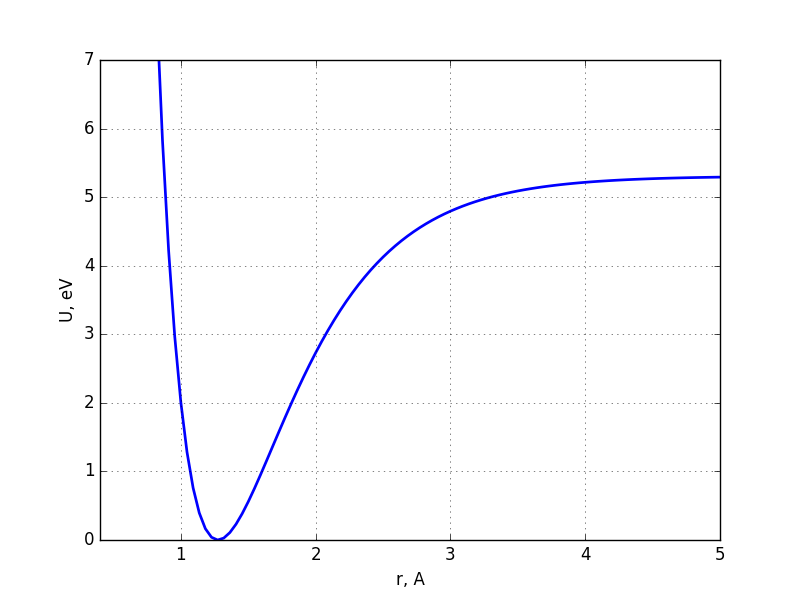
\includegraphics[scale=0.5]{pictures/potential.png}
	\caption{График функции потенциальной энергии}
\end{figure}

\section{Распределение интенсивностей во вращательной структуре}

\begin{gather}
	\frac{N_J}{N_0} = \lb 2 J + 1 \rb \exp \lb -\frac{B c h J ( J + 1 )}{kT} \rb \notag \\
	\frac{1}{N_0} \frac{d N_J}{d J} = 0 \quad \implies \quad J_{max} = \sqrt{ \frac{k T}{2 B h c} } - \frac{1}{2} \notag
\end{gather}

\begin{figure}[!ht]
	\centering
	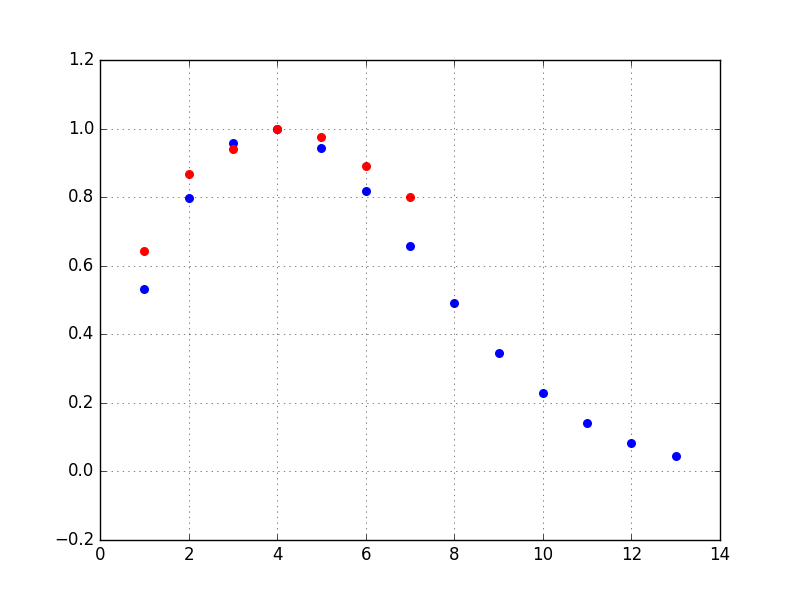
\includegraphics[scale=0.5]{pictures/population.png}
	\caption{Относительная заселенность уровней (синий);  \newline относительная интенсивность переходов в экспериментальном спектре (красный)}
\end{figure}

\clearpage
\section{Расчет колебательно-вращательных переходов изотопозамещенной молекулы}

\begin{table}[!ht]
	\centering
	\begin{tabular}{|c|c|c|c|}
		\hline
		& Переход & $\nu$(расч.) & $\nu$(эксп.) \\
		\hline
		Молекула $HCl$ & $7 \rightarrow 6$ & $2721.18$ & $2727.7796$ \\
		$\rho = 0.7172$ & $6 \rightarrow 5$ & $2747.34$ & $2752.0353$ \\
		$\omega_e (\textup{расч.}) = 2990.728 \, \textup{см}^{-1}$ & $5 \rightarrow 4$ & $2772.63$ & $2775.7609$ \\
		$\omega_e (\textup{эксп.}) = 2990.9460 \, \textup{см}^{-1}$ & $4 \rightarrow 3$ & $2797.06$ & $2798.9432$ \\
		$\omega_e x_e (\textup{расч.}) = 52.199 \, \textup{см}^{-1}$ & $3 \rightarrow 2$ & $2820.63$ & $2821.5691$ \\
		$\omega_e x_e (\textup{эксп.}) = 52.8186 \, \textup{см}^{-1}$ & $2 \rightarrow 1$ & $2843.33$ & $2843.6254$ \\
		$B_e (\textup{расч.}) = 10.593 \, \textup{см}^{-1}$ & $1 \rightarrow 0$ & $2865.16$ & $2865.0991$ \\
		$B_e (\textup{эксп.})  = 10.5934 \, \textup{см}^{-1}$ & $0 \rightarrow 1$ & $2906.24$ & $2906.2479$ \\
		$B^\prime (\textup{расч.}) = 10.053 \, \textup{см}^{-1}$ & $1 \rightarrow 2$ & $2955.20$ & $2925.8977$ \\
		$B^\prime (\textup{эксп.}) = 10.136223 \, \textup{см}^{-1}$ & $2 \rightarrow 3$ & $2943.86$ & $2944.9146$ \\
		$B^\dprime (\textup{расч.}) = 10.458 \, \textup{см}^{-1}$ & $3 \rightarrow 4$ & $2961.37$ & $2963.2864$ \\ 
		$B^\dprime (\textup{эксп.}) = 10.440254 \, \textup{см}^{-1}$& $4 \rightarrow 5$ & $2978.02$ & $2981.0013$ \\ 
		& $5 \rightarrow 6$ & $2993.80$ & $2998.0473$ \\
		& $6 \rightarrow 7$ & $3008.72$ & $3014.4130$ \\ 
		& $7 \rightarrow 8$ & $3022.77$ & $3030.0870$ \\
		\hline
	\end{tabular}
\end{table}

\section{Литература}

\begin{enumerate}
	\item Rank, D. H., Eastman, D. P., Rao, B. S., Wiggins, T. A. (1962). Rotational and vibrational constants of the HCl$^{35}$ and DCl$^{35}$ molecules. J. of the Opt. Soc. of Am., 52, 1.  
\end{enumerate}

\end{document}